%!TEX root = main.tex
\section{Results}

•Objective presentation of key results, without interpretation (text and tables
and figures)
•Important negative results should also be reported

\begin{figure}[H]
  \centering
  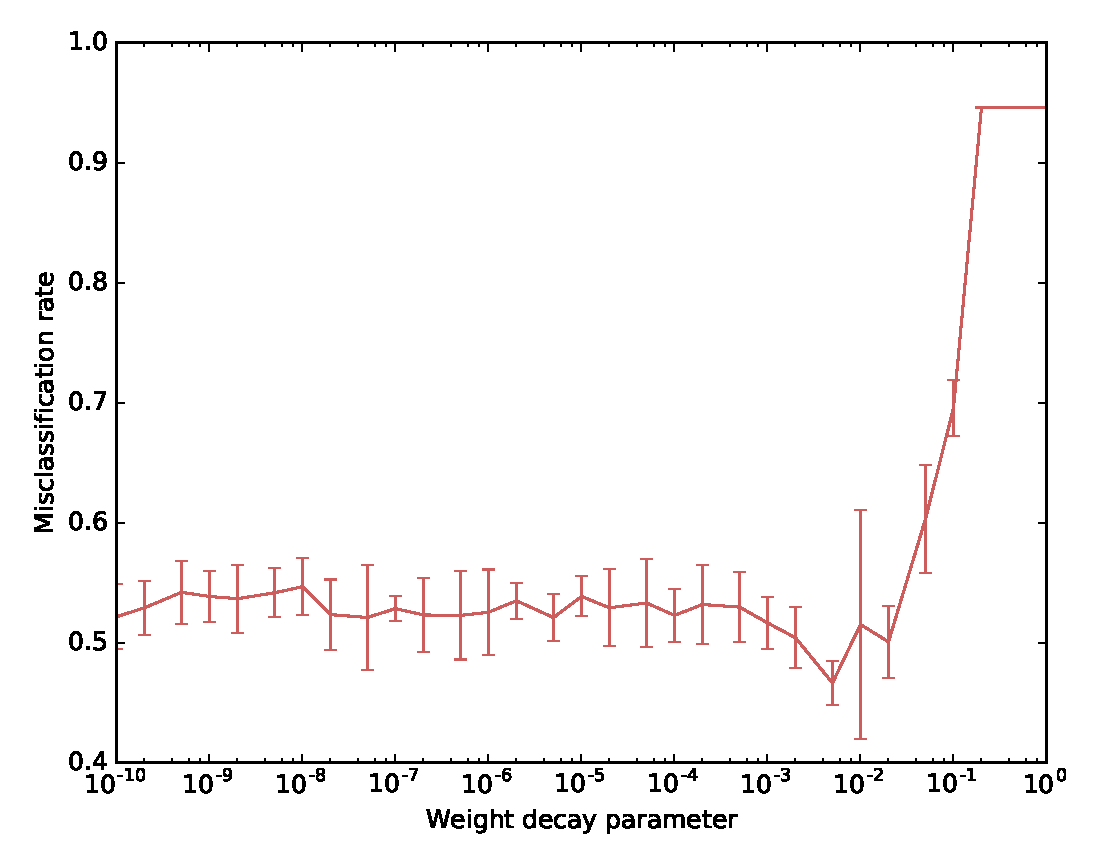
\includegraphics[width=0.4\textwidth]{plots/reg_opt_dieleman_speaker_elsdsr}
  \caption{Misclassification rate confidence interval for different weight decay parameter values, for the speaker classification problem on the ELSDSR dataset, obtained using $5$-fold cross-validation.}
  \label{fig:reg_opt}
\end{figure}

In order to test whether weight decay has an significant improvement to the performance, an independent two-sampled t-test is used (assumes equal variance). Given the mean misclassification rates $\mu_1$ and $\mu_2$ for the regularization parameter being $0$ and $5 \cdot 10^{-3}$ respectively, our null-hypothesis is defined as $\mu_1$ and $\mu_2$ being different
\begin{equation}
\begin{aligned}
\text{H}_\text{0} \, &\text{:} \, \mu_1 \ne \mu_2 \\
\text{H}_\text{a} \, &\text{:} \, \mu_1 = \mu_2.
\end{aligned}
\end{equation}
The resulting p-value for a two-sided t-test is $p = 0.0030$ i.e. the null-hypothesis is rejected and our alternative hypothesis is confirmed, hence we cannot say that adding weight decay has significant performance improvement with a $95\%$ significance level.
